%% LyX 2.3.0 created this file.  For more info, see http://www.lyx.org/.
%% Do not edit unless you really know what you are doing.
\documentclass[english,it,preprint]{iucr}
\usepackage{mathpazo}
\usepackage[T1]{fontenc}
\usepackage[latin9]{inputenc}
\usepackage[a4paper]{geometry}
\geometry{verbose,tmargin=2cm,bmargin=2cm,lmargin=2cm,rmargin=2cm}
\setlength{\parskip}{\medskipamount}
\setlength{\parindent}{0pt}
\usepackage{array}
\usepackage{graphicx}

%%%% Copied from IUCr.cls to get proper cross-references
  \renewcommand{\thepart}{%                      % Section numbering
     \arabic{part}}
  \renewcommand{\thesection}{%                   % Section numbering
     \arabic{part}.\arabic{chapter}.\arabic{section}}
  \renewcommand{\thesubsection}{%                % Subsection numbering
     \if@ppend@x A\fi%
      \arabic{part}.\arabic{chapter}.\arabic{section}.\arabic{subsection}}
  \renewcommand{\thesubsubsection}{%             % Subsubsection numbering
     \if@ppend@x$\mathrm{A}$\fi%
     $\arabic{part}.\arabic{chapter}.\arabic{section}.\arabic{subsection}%
     .\arabic{subsubsection}$}

\makeatletter

%%%%%%%%%%%%%%%%%%%%%%%%%%%%%% LyX specific LaTeX commands.
%% Because html converters don't know tabularnewline
\providecommand{\tabularnewline}{\\}

%%%%%%%%%%%%%%%%%%%%%%%%%%%%%% Textclass specific LaTeX commands.
\usepackage{harvard}

%%%%%%%%%%%%%%%%%%%%%%%%%%%%%% User specified LaTeX commands.
\renewcommand{\harvardurl}[1]{\textbf{URL:} \textit{#1}}
\part{1}
\chapter{4}
\parttitle{Concepts and specifications}

\makeatother

\usepackage{babel}
\begin{document}
\title{Construction and interpretation of CIF dictionaries}

\author[a]{J. R.}{Hester}
\author[b]{N.}{Spadaccini}
\aff[a]{Australian Nuclear Science and Technology Organisation \country{Australia}}
\aff[b]{University of Western Australia, \country{Australia}}


\maketitle

\section{Introduction}

CIF dictionaries provide a machine- and human- readable description
of the possible contents of arbitrary datasets. Machine-readability is
achieved in part by use of a controlled vocabulary, which is referred to here as
a "dictionary definition
language" (DDL). The set of words contained in a DDL vocabulary, or "attributes",  
are generally limited in CIF DDLs to those
necessary for
reliable data ingestion into
software and for long-term archiving. More 
recent frameworks for describing data,
such as the Web Ontology Language (OWL) \cite{owl2} and
the Resource Description Framework (RDF) \cite{rdf}, are much broader in scope,
providing vocabulary for describing a wide range of logical relationships between
data items and facilitating the linking of independently-developed
vocabularies to create a semantic web. The more minimal CIF approach assumes that, where
relevant, such information is already encapsulated in correctly-functioning software
handling the data.

Section \ref{subsec:The-dictionary-data-model} describes the
way in which arbitrary data are modelled by the CIF dictionary. Section \ref{sec:DDLm}
describes the DDLm dictionary definition language used in IUCr dictionaries,
and section 1.4.3 describes the DDL2 dictionary definition language
used in dictionaries related to protein crystallography.  Advice
on creating dictionaries is found in Section 2.1. 

\subsection{\label{subsec:The-dictionary-data-model}The dictionary data model}

A CIF dictionary models
data as a collection of \textit{data values}, one or more of which is
associated with a \textit{data name} to form a \textit{data item}. The dictionary contains definitions
for each of these data names, thus allowing interpretation of the
associated data values. Such a collection
of data name definitions may be viewed as a simple \textit{ontology}
in the sense of \citeasnoun{Gruber1993}. In files constructed according
to the CIF syntax (Section 1.2), these
data names appear explicitly together with their associated values.

A CIF dictionary data name definition always contains a plain text,
human-readable description of the meaning of the data name. These descriptions are a typical
starting point for a CIF dictionary user, as through the descriptions the data
name is linked into general scientific discourse.

CIF dictionaries use the relational model \cite{codd} to describe the
relationships between data values. The relational model arranges data 
into "relations", which are simply tables with certain properties.
Simple properties include:
\begin{enumerate}
\item Column names are unique
\item Changing row or column order does not change the meaning
\item Rows are not repeated
\item Values in a given column have the same type
\end{enumerate}

Table \ref{tab:CIF-and-equivalent}
describes how terms used in the CIF context relate to terms
used in relational modelling, and the following paragraphs give a brief
overview of those aspects of the relational model relevant to CIF
dictionaries.

The data in each column of a relation must have the same \textit{type}.
A type labels a domain from which the values in that column can 
be drawn, for example the set of real numbers, the set of non-zero integers, 
or a list of text options. A CIF dictionary assigns a particular type 
to every data name. 

Every relation has a "key". A key is a subset of column names whose values in
any given row can be used to distinguish that row from all other rows in the
relation. The particular values for a given row are termed the "key value" or "value of
the key". In a CIF context, the key is therefore a set of one or more data names. 
Each column in a relation is a mathematical function of the key, mapping the
values taken by the key data names to the values in that column. Section 2.1 includes
a discussion of how to select or create key data names when writing dictionaries.

In the CIF dictionary context, a "category" is the collection of data names that 
appear together in a table. In some discussions, "category" is also used
to describe the whole table; the distinction will be clear from the context.

\begin{table}
\begin{tabular}{lll}
CIF & Relational Model & Alternative Name\tabularnewline
\hline 
category & relation & table\tabularnewline
packet & tuple & row\tabularnewline
key & key & base\tabularnewline
data name & attribute & column\tabularnewline
\end{tabular}

\caption{ \label{tab:CIF-and-equivalent} Comparison between CIF and equivalent relational terminology}

\end{table}

It follows from the above discussion that the information provided in a 
dictionary for each data name
must at minimum include: (i) a plain text description; (ii) which
category the data name belongs to; (iii) the type of the data values.
Category definitions should identify the key data names for the category.
The dictionary definition languages used by CIF and described below
prescribe further attributes to ensure that inter-category relationships
and constraints can be expressed, and that auditing and fine-grained
validation are possible.

In essence, CIF dictionaries model data as lists of data values associated
with data names. The dictionary arranges these lists into the columns of one or
more relations. Importantly, there is no 
intrinsic DDL requirement that data are expressed using a format that provides tabular
layout; data values must simply be
associated with data names with consistent ordering. Nor is there a requirement
that the data name appears together with the data; it is sufficient that a data name can be
associated with a value appearing at a particular logical location. For
example, a text file containing columns of numbers can be 
correctly interpreted after specifying which data names are associated 
with each column.
By adopting this general approach to data description, CIF dictionaries
can describe data encapsulated in a wide variety of data formats, for example
JSON (Section 1.6) or HDF5 \cite{Hester2016},
although in practice CIF dictionary use has focused on the CIF format.

Note that in the following material references to
tables and data names within a data file assume that the appropriate data name
assignments and arrangement of columns according to the dictionary specifications
have taken place.

\subsubsection{Comparison with the CIF syntax data model}

The dictionary data model
described here can be described as a development of the CIF syntax data model (Section 1.2.2). 
Application of the dictionary data model to the CIF syntax data model restricts the data names 
that can appear together in CIF loops,
at the same time as allowing a greater variety of data value types. Therefore, a CIF dictionary must
be consulted in order to determine both the semantic type of a data value appearing in
a CIF file, and which data names belong together in a category and therefore should appear in
the same loop.

The data blocks and save frames found in the CIF syntax have no correlates within
the dictionary model. Instead, data blocks are notionally merged to form the complete
data set as discussed in Section 3.1.

\subsection{Dictionary definition languages}

A wide variety of approaches to describing data
meet the minimal data name description requirements outlined in the
previous section. For example, natural text in a single document is often 
used to describe a file format and data item locations. If such 
dictionaries are instead structured according to
a regular syntax and draw from a well-defined,
small vocabulary, the dictionary becomes machine-actionable, allowing
among other things validation of data file contents and transformation
to a variety of text formats. CIF dictionaries adopt this machine-friendly
approach, and use CIF syntax (Section 1.2) so that the same programming code can
be used to read both CIF data files and CIF dictionaries.
Section 7.1 provides historical background on this choice. 

The small vocabulary used by CIF dictionaries, 
the "dictionary definition language" (DDL), contains no information about a discipline; 
rather, it defines the data names that can be used to describe a discipline. 
If the contents 
of a dictionary are metadata, or data about data,  
the contents of the DDL are meta-metadata, the data defining the metadata. 
By design CIF DDLs are quite generic. They define attributes that describe 
the general features of a data name, such as a textual description, a data type, 
a set of examples, or a range or discrete set of permissible values. Consequently, 
data modelling using a DDL can be applied in many fields. 

Syntactically, a CIF dictionary is composed of a sequence of relatively
short save frames collected within a single data block. Each save
frame contains the definition of a single data name or category (Figure
\ref{fig:item-att-example}). The definition within each save frame
is built up using the usual CIF tag - value and loop constructions.
In the context of a CIF dictionary the tags are known as \textit{attributes},
and form the controlled vocabulary required for machine readability.
For historical reasons (see Section 7.1),
two similar DDLs are currently in use, DDL2 and DDLm. Broadly speaking, dictionaries
for use in chemical crystallography are written in DDLm, while the DDL2 language
is used in protein crystallography (mmCIF, Chapter 2.10) and related
areas. Data names defined in dictionaries using either DDL can be mixed together, for
example by using imgCIF (Section 2.11) to describe raw data from a small-molecule
single crystal experiment. An earlier DDL (DDL1) is no longer in use, but is included
in Section 7.3 for historical reference.

\section{DDLm\label{sec:DDLm}}

Like all dictionary definition languages, DDLm includes attributes
to define the fundamental category relationships described in the
previous section. In addition, machine-executable algorithms may be
included in definitions, facilitating the automatic evaluation of
derivable data values directly from other data and definition information,
and taking advantage of the simple structure of the data model. DDLm
also includes a templating system for sharing of definitional information
across disparate dictionaries to enable coordinated operation and
to reduce duplication.

DDLm introduces distinctions between measured or observed data and
derived data, where derived data can be calculated from other data
items. For database archiving, the presence of derivative items in
the experimental record has both advantages and disadvantages. In
a well-defined domain, derivative data is in a sense redundant since
it can be recalculated; on the other hand, the original derivative
values provide a means to validate related data. When data interdependencies
are precisely recorded in a dictionary, the option to not archive
the derivative data exists. 

A DDLm dictionary describes a complete data set consisting of a
collection of data blocks. A "data block" is any collection of
data items that is encapsulated in some way. For example, when using 
data files in CIF format, the complete data set may consist of
single or multiple CIF data blocks. Note that application of DDLm to multi-block data sets is a 
relatively recent expansion of the standard, and most CIF usage focuses
on single-block data sets.
In the following discussion, the terms "data collection" and "data set"
are used interchangeably to refer to the entirety of the data described
by the dictionary. 

\subsection{The DDLm data model}

Like all DDLs presented here, DDLm attributes work within the relational
model described in Section \ref{subsec:The-dictionary-data-model}.
DDLm additionally distinguishes certain special cases and provides
mechanisms for building up ontologies from multiple dictionaries.

\subsubsection{\label{subsec:Loop-and-Set}Loop and Set categories}

Categories are classified as either 'Loop' or 'Set' categories.
Data names belonging to a 'Loop' category may be assigned one or more values within a data block,
whereas data names from 'Set' categories may only take a single value. 'Set'
categories, being one-row relations, do not require key data names to be defined,
as there is no need to distinguish rows. However, if items from a Set category
might appear in multiple data blocks forming part of a data collection, a key data name for
that category must be defined. Information on using DDLm to describe multi-block datasets is
given in Section 3.1.

\subsubsection{\label{subsec:Nested-categories}Category and definition hierarchy}

DDLm arranges categories into a hierarchical tree, in which every
category has a 'parent' category. The root of the tree (the ultimate
parent) is called a 'Head' category and has a special significance
when combining dictionaries (see \ref{subsec:Import-detail}). No data
names are contained within a Head category, and all 'Set' categories must be
children of this 'Head' category. 'Loop' categories may
be children of either the 'Head' category, or of another 'Loop' category. 
In the latter case the two categories can in principle be interpreted
as a single 'Loop' category. The key data names of the parent category
each correspond to a key data name in the child category, and the values of either set of 
key data names can be used for the purpose of identifying rows
in either category. A
data file may present data from such categories either in a single
table, or as two separate tables. In relational database terms, the
merged category is the result of a left outer join of the parent category
with the child category using the key data names. 

Such category splitting is useful in situations where some data items from
a category are present for only a minority of the category
packets. For example, for a given dataset only a few atoms may have
refined anisotropic displacement parameters, and so anisotropic displacements
are more compactly presented in a separate table where only the relevant
atoms are listed. Similarly, in magnetic structures
atomic moments are not relevant for non-magnetic atoms, even though atomic moments
depend on the atom site and thus can
be tabulated together with other atomic properties like position and
displacement parameters. The magnetic properties are therefore
placed into a child category of the atom site category to allow data
file creators to present the magnetic properties of the atomic sites
in a separate table. This improves data file concision as otherwise
the rows for atoms that have no values defined for the child data
names would need to include placeholder null values.

\subsubsection{Data name relationships}

Values of a data item in one category will sometimes draw upon the
same set of values as some other data item, usually found in a separate
category. This situation arises, for example, when specifying the
atoms between which a bond is formed: the values of the data items
identifying each end of the bond must correspond to values of the
atom site labels, which are listed in a different category. When such
relationships occur between data names forming the keys
of different categories the categories themselves become linked, allowing
each row of one category to be associated with
a unique row of the other category.

A different type of link between data names arises between a value
and its standard uncertainty. DDLm provides a mechanism to specify
that one data item holds the standard uncertainty (SU) of another data item.
When using CIF formats, which allow the SU to be presented as part of a
data value, this separate SU data name is assigned the SU value (see
Table \ref{tab:DDLm-derive-CIF}). Where 
both an appended SU and a separate SU data item are present for a data item, the
values must agree. CIF users should also note that appending SU may
not be possible in cases where an integer data type has an SU that is smaller
than one (for example an SU of 0.8 on a value of 2), in which case the
explicit SU data name is available.

\subsection{The DDLm attributes}

A DDLm dictionary is structured using save frames inside an enclosing data block (Figure
\ref{fig:ddlm-dictionary-structure}).
Attributes appearing outside the save frames are called "dictionary" attributes.
The discussion of DDLm attributes below has been divided into those relevant to the
item, category and dictionary levels. The dictionary defining the
attributes (itself a DDLm dictionary) is presented in Section 3.2,
which may be used as a reference.

\begin{figure}

\caption{Example of DDLm dictionary structure using an extract from the twinning
dictionary (Section 2.4). Information about the dictionary itself is
included in the enclosing data block, with save frames containing
the definitions of (i) a 'Head' category (ii) one child category (iii)
a data name.}

\label{fig:ddlm-dictionary-structure}

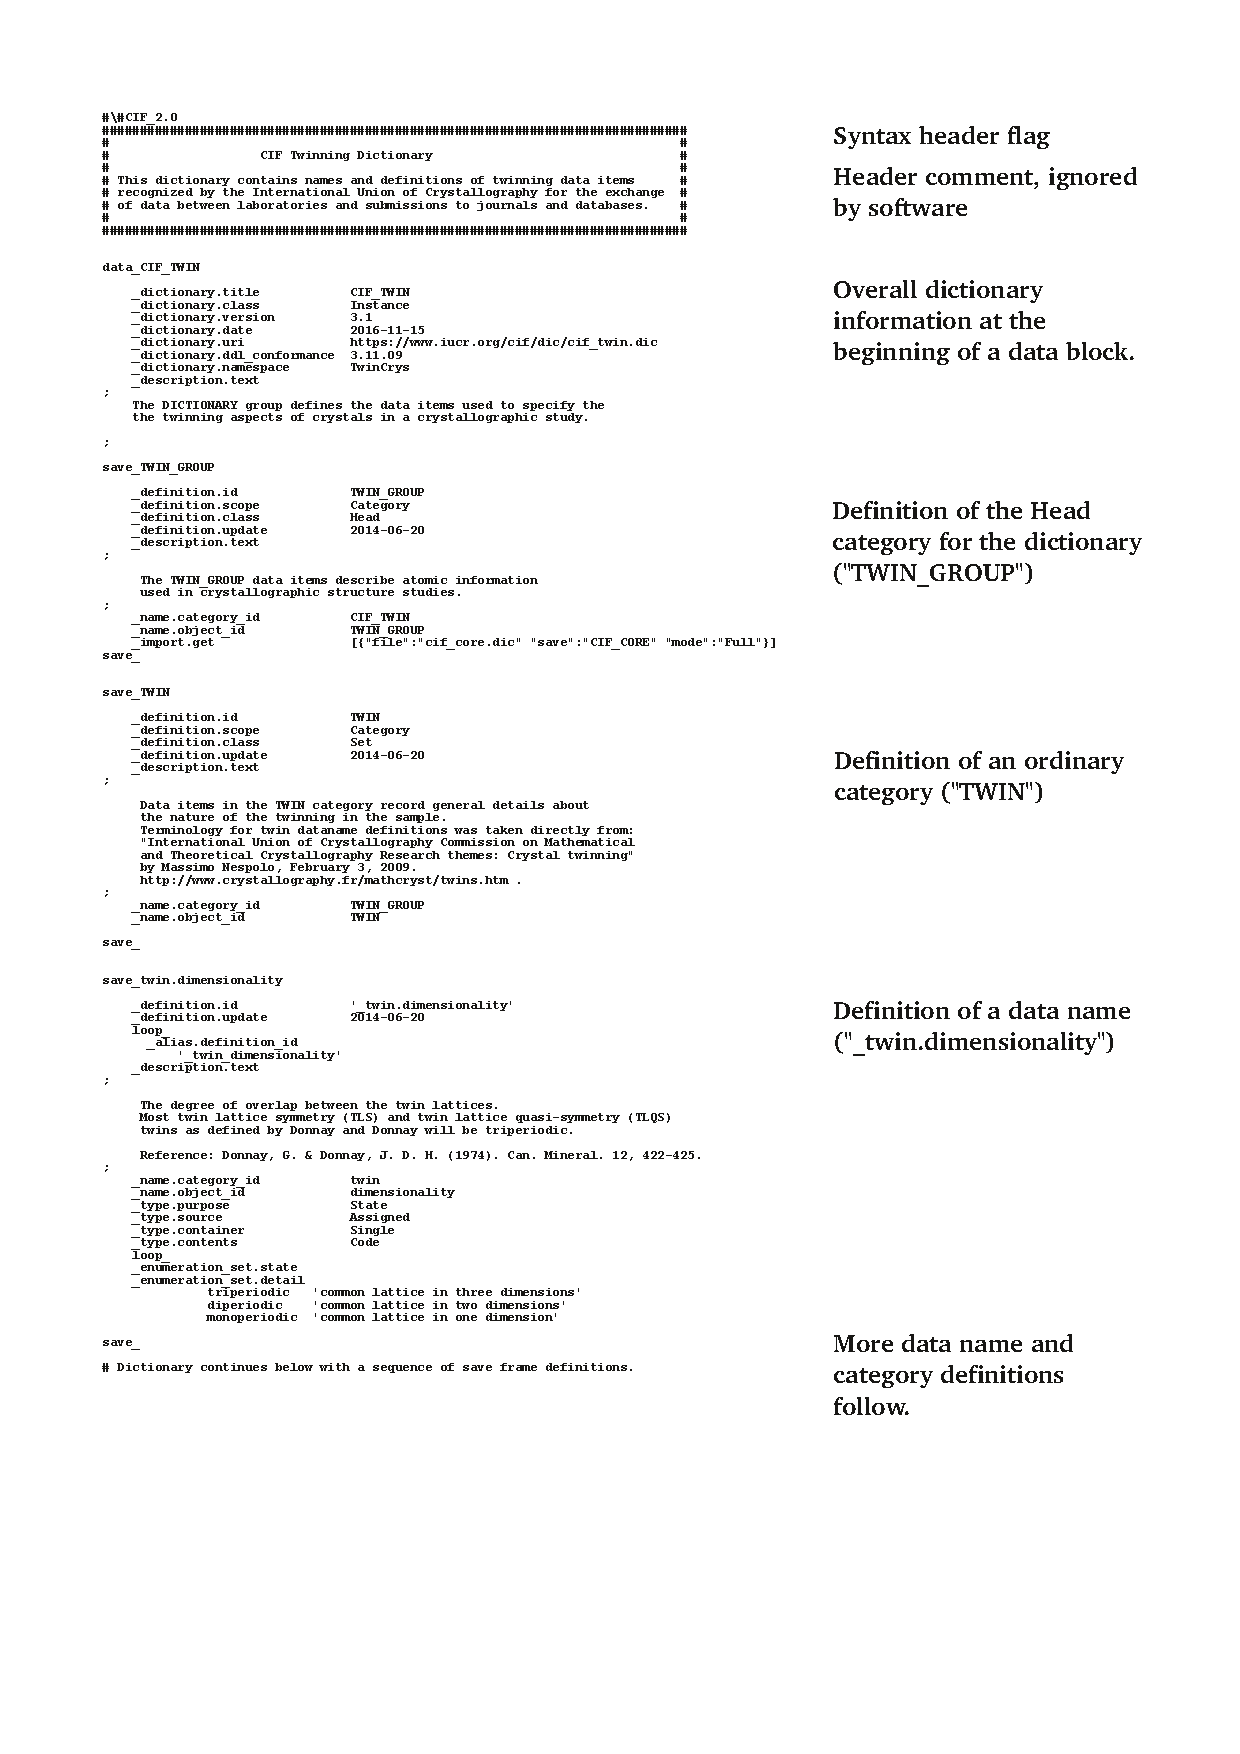
\includegraphics[width=1\textwidth]{Dictionary-structure-diagram}
\end{figure}

\subsubsection{Item-level attributes}

DDLm attributes intended for item definitions are listed in Table
\ref{tab:item-atts}. Attributes whose default values correspond to item
definitions (\cifname{_definition.class},\cifname{_definition.scope}) have been omitted. Figure \ref{fig:item-att-example} contains
a typical definition using some common attributes.

\begin{table}
\begin{tabular}{>{\raggedright}p{0.5\textwidth}>{\raggedright}p{0.5\textwidth}}
Attribute & Description\tabularnewline
\hline 
\texttt{\textbf{\scriptsize{}\_alias.definition\_id}} & Historical equivalents to the defined data name\tabularnewline
\texttt{\textbf{\scriptsize{}\_definition.id}} & The data name being defined\tabularnewline
\texttt{\textbf{\scriptsize{}\_definition.update}} & When the definition was last edited\tabularnewline
\texttt{\textbf{\scriptsize{}\_description.text}} & A full description of the data name's meaning\tabularnewline
\texttt{\textbf{\scriptsize{}\_description\_example.case}} & An example value\tabularnewline
\texttt{\textbf{\scriptsize{}\_description\_example.detail}} & An explanation of the example case\tabularnewline
\texttt{\textbf{\scriptsize{}\_enumeration\_set.state}} & Used to list possible values of a data name\tabularnewline
\texttt{\textbf{\scriptsize{}\_enumeration\_set.detail}} & Explanation of value given by \_enumeration\_set.state\tabularnewline
\texttt{\textbf{\scriptsize{}\_enumeration.default}} & A value that can be used when the data name is absent from a data
file\tabularnewline
\texttt{\textbf{\scriptsize{}\_enumeration.def\_index\_id}} & The data name whose value is used to look up a default value for the
defined data name in the ENUMERATION\_DEFAULT loop\tabularnewline
\texttt{\textbf{\scriptsize{}\_enumeration\_default.index}} & A value that is used to index into an ENUMERATION\_DEFAULT loop\tabularnewline
\texttt{\textbf{\scriptsize{}\_enumeration\_default.value}} & The value corresponding to an \_enumeration\_default.index\tabularnewline
\texttt{\textbf{\scriptsize{}\_enumeration.range}} & Inclusive range of
allowed values\tabularnewline
\texttt{\textbf{\scriptsize{}\_import.get}} & Insert additional attributes from the referenced block\tabularnewline
\texttt{\textbf{\scriptsize{}\_method.purpose}} & The purpose of the dREL expression\tabularnewline
\texttt{\textbf{\scriptsize{}\_method.expression}} & An expression written in dREL that can be used to calculate values
of the defined data name from other values in a data file\tabularnewline
\texttt{\textbf{\scriptsize{}\_name.category\_id}} & The category this item belongs to\tabularnewline
\texttt{\textbf{\scriptsize{}\_name.object\_id}} & The unique part of the name within the category\tabularnewline
\texttt{\textbf{\scriptsize{}\_name.linked\_item\_id}} & A data name whose values the defined data name draws from, or else
the data name for which the defined data name is the su. \tabularnewline
\texttt{\textbf{\scriptsize{}\_type.container}} & The type of compound value, or else 'Single'\tabularnewline
\texttt{\textbf{\scriptsize{}\_type.contents}} & The type of individual values\tabularnewline
\texttt{\textbf{\scriptsize{}\_type.dimension}} & The dimension of a compound value\tabularnewline
\texttt{\textbf{\scriptsize{}\_type.purpose}} & The purpose for which this data name is used\tabularnewline
\texttt{\textbf{\scriptsize{}\_type.source}} & The origin of the data value\tabularnewline
\texttt{\textbf{\scriptsize{}\_units.code}} & The units of measurement of the data name values\tabularnewline
\end{tabular}

\caption{\label{tab:item-atts}Common attributes used in item definitions}
\end{table}

\begin{figure}
\caption{\label{fig:item-att-example}A definition for \cifname{_diffrn_source.device}
showing use of the most common attributes}

\begin{boxedcifdefblock}
\begin{ciflisting}
save_diffrn_source.device
_definition.id '_diffrn_source.device'
_definition.update 2018-02-26
_description.text 
;
Enumerated code for the device providing 
the source of radiation.christogrozev
;
_name.category_id diffrn_source
_name.object_id device
_type.purpose State
_type.source Assigned
_type.container Single
_type.contents Text
loop_
_enumeration_set.state
_enumeration_set.detail
tube 'sealed X-ray tube' 
nuclear 'nuclear reactor' 
spallation 'spallation source' 
elect-micro 'electron microscope' 
rot_anode 'rotating-anode X-ray tube' 
synch synchrotron 
save_
\end{ciflisting}
\end{boxedcifdefblock}
\end{figure}

The \cifname{_definition.id} attribute is given the name of the data
name being defined, and is conventionally the first attribute listed
in a definition block. The category to which a data name belongs
is given by \cifname{_name.category_id}, which will usually match
the part of the data name preceding the period character (see point
\ref{enu:Data-names-period} in \ref{subsec:Stylistic-considerations}).
The part of the data name that follows the period conventionally matches
\cifname{_name.object_id}. These two attributes taken together are
the way in which a data name is referenced in dREL methods (see Section
1.5). 

It is unfortunately inevitable that identical meanings will be assigned
to different data names over time. Data name \cifname{_alias.definition_id}
is used to list alternative data names that refer
to an identical concept. The \cifname{_definition.update} attribute
is used as basic audit information to track any changes to definitions.

A free-text description of a data name's meaning is provided in the
value of the \cifname{_description.text} attribute. This description
is intended for human readers and typically will be processed automatically
for display online or in printed documents, as has been done for the
dictionary sections of this volume.  To this end, dictionary authors 
may use the markup conventions
described in Section 1.2. In item 
definitions, \cifname{_description_example.case}
provides example values for the data item as they would appear in a CIF syntax file. \cifname{_description_example.detail}
is used to explain in more detail, if necessary, the correct
interpretation of the given example. Units are specified using \cifname{_units.code},
whose values are unit abbreviations drawn from a list provided in
the DDLm attribute dictionary (see Section <ref to units.code> for
the full list).

Information on the type of values taken by a data name are provided
in \cifname{_type.contents} and \cifname{_type.container}. When
\cifname{_type.container} is Single, \cifname{_type.contents} is
assigned a value from a simple list (see <ref to type.contents definition>)
that describes the defined data name's type. For compound data values,
which are usually arrays or matrices, \cifname{_type.container} will
take the appropriate value, and then \cifname{_type.contents} describes
the type of each element of the container. \cifname{_type.dimension}
can be used to specify the size of such compound data values. When
dealing with case insensitive text data types, values that compare equal
under Unicode canonical caseless matching are considered equivalent.

Use of DDLm dictionaries with a given
data format requires specification of the mapping between values as they 
appear in that format and the DDLm types as described by the above attributes. 
Such specifications always
supercede any implicit typing provided by the format, although
DDLm types should be matched to the most similar syntactical types 
where possible to minimise the possibility of programmer error.
Table \ref{tab:DDLm-derive-CIF} describes this mapping for
the CIF syntax. This description overrides any
implicit data typing (see 1.2.4.2) and is the default specification
for using DDLm dictionaries with text-based file formats. 

\begin{table}
\begin{tabular}{>{\raggedright}p{0.2\textwidth}l>{\raggedright}p{0.5\textwidth}}
DDLm type & Example & Derivation from CIF value\tabularnewline
\hline
Text & Fe3 & no change\tabularnewline
Dimension & [3, 4] & interpret string as square-bracket delimited array of integers separated by commas with optional internal whitespace\tabularnewline
Range & 0:10 & Split CIF value on ':' character and interpret resulting two values as numeric min,max.\tabularnewline
Integer, Real & 3.14 & Interpret string according to 1.2.4.2.3\tabularnewline
Integer, Real with uncertainty & 1.72(15) & Interpret string according to 1.2.4.2.3, 
assigning the uncertainty 
to the linked SU data name\tabularnewline
Imag & 2.10(3)j & Final character of string should be 'j'; remainder of string interpreted as number and multiplied by $i$\tabularnewline
Complex & 1-3j & CIF string should have form 'a $\pm$ bj' (whitespace optional) where $a$ and $b$ are interpreted as numbers\tabularnewline
List, Array, Matrix & [1 2 3] & CIF2 list type with elements interpreted as per the present table\tabularnewline
Table & \{a:2 b:3\} & CIF2 table type with keys unchanged and values interpreted as per the present table\tabularnewline

\hline 

\end{tabular}

\caption{ \label{tab:DDLm-derive-CIF} Deriving DDLm types from CIF data values. Type
'Text' refers to all DDLm types whose final form is a sequence of characters. 
Any transformations specified by Table 1.2.4.2.1 must be performed first, together with removal of any enclosing
quotes. Numeric interpretation is according to 1.2.4.2.3. List, Array, Matrix and Table
data types are not available in CIF1 format}

\end{table}

Certain data values may be drawn from a finite set of options. In such
cases, \cifname{_type.contents} is assigned a value corresponding
to the type of these values (usually 'Text') and a loop over \cifname{_enumerated_set.state}
and \cifname{_enumerated_set.detail} is added to the definition.
The \cifname{_enumerated_set.state} column lists the finite set of
options for the data name's value, and the \cifname{_enumerated_set.detail}
column gives a textual explanation of the meaning of each option, 
intended for human readers. Note that where a case-insensitive type has been
indicated in \cifname{_type.contents}, the case of the options is not 
significant.

\cifname{_enumeration.range} is used to specify the allowed maximum and/or minimum values of an item. 
If a standard uncertainty is
associated with a value, reported values may lie outside this range.

When the values that a data name can take are drawn from the values
taken by some other data name (for example, the label for the atoms at each end
of a bond described in the \cifname{geom_bond} category must be drawn
from the set of atom labels described by \cifname{_atom_site.label}),
the data name providing the source of values is specified using attribute
\cifname{_name.linked_item_id}. This attribute is also used to specify
that the data name being defined is the standard uncertainty for the
data name given as the value of \cifname{_name.linked_item_id}. These
two uses of this attribute are disambiguated by setting values for
\cifname{_type.purpose}: 'Link' for the former case (see below),
and 'SU' for the latter.

A default value for a data name is specified using \cifname{_enumeration.default},
with the meaning that such values may be assumed by software if a
data name is missing. Dictionary authors should only provide such
default values where they can be certain that (i) no situation can
arise for which the value is truly unknown, and (ii) it will never
be the case that a value is known to be a non-default value but is
omitted from the data file. In practice, such situations are rare
and this attribute should be used sparingly, if at all. 

Tables of constants can be incorporated into a dictionary, both as
a standard reference and to facilitate automated derivation of data
values using dREL (Section 1.5). To support such usage, constants
are tabulated using \cifname{_enumeration_default.index} and \cifname{_enumeration_default.value}
(Figure \ref{fig:using-default-enumerations}). \cifname{_enumeration_default.index}
provides a code through which a value in \cifname{_enumeration_default.value}
can be selected. A definition can then set \cifname{_enumeration.def_index_id}
to the data name whose value should be used to look up this loop
to find a default value to use when no value is provided in the data
file. In the example shown in Figure \ref{fig:using-default-enumerations},
the atomic mass of an atom is assigned based on the atomic symbol
using this mechanism. To avoid clutter in the dictionary, long tabulations
are usually stored in a separate file and the import mechanism used
to insert them into the appropriate definitions. Note that this context
for determining default values is qualitatively different to specifying
a default value for a data name whose value might change from experiment
to experiment and therefore use of this mechanism is not subject to
the same strong caveats discussed above for \cifname{_enumeration.default}.

\begin{figure}

\caption{Using default enumerations. In the definition of \cifname{_atom_type.atomic_mass},
the value of \cifname{_atom_type.symbol} is used to look up the \cifname{ENUMERATION_DEFAULT}
loop to assign a default value for the atomic mass.}

\label{fig:using-default-enumerations}

\begin{boxedcifdefblock}
\begin{ciflisting}
save_atom_type.atomic_mass
_definition.id                 '_atom_type.atomic_mass'
_definition.update             2012-11-20
_description.text                        
;
     Mass of this atom type. 
;
_name.category_id              atom_type
_name.object_id                atomic_mass 
_type.purpose                  Number
_type.source                   Assigned
_type.container                Single
_type.contents                 Real
_enumeration.def_index_id      '_atom_type.symbol'
_units.code                    dalton
     loop_
           _enumeration_default.index
           _enumeration_default.value
      H     1.008
      D     2.008
      H1-   1.008
      He    4.003
      Li    6.941
      Li1+  6.941
      Be    9.012
\#...
save_
\end{ciflisting}
\end{boxedcifdefblock} 
\end{figure}

The role and source of a data value is specified using \cifname{_type.purpose}
and \cifname{_type.source}. These attributes take values from lists
specified in the DDLm attributes dictionary (<ref to Section 3.2>).
As mentioned above, \cifname{_type.purpose} is used when identifying
data names that act as the standard uncertainties for another data
name. Similarly, any data name for which \cifname{_type.purpose} is 'Measurand'
is required to have a data name defined corresponding to its standard uncertainty.
Conventionally this data name is formed by appending \texttt{\_su}.
Note that a value of 'Key' for \cifname{_type.purpose} must
only be used where values of the data name form part of the category
key \textit{and} contain no other information. So, for example, \cifname{_atom.label}
is not assigned a \cifname{_type.purpose} of 'Key', despite being
the category key for category 'atom', as the atom label consists of
a number of components carrying meaning. 

The \cifname{_type.source} attribute records the source of values for a particular data
name as viewed by the dictionary authors. For example, in some applications
the value of a data name may be 'Recorded', which means
that it is measured or cannot be derived from other entries in the data
file. If the dictionary authors had instead chosen to define data
names that allow the original data name to be calculated, \cifname{_type.source}
for that same data name would be 'Derived'. The \cifname{_type.source}
value 'Assigned' should only be used where a choice has been made.

Finally, methods for deriving the value of a data name from other
values can be expressed using a dREL language expression as the value
of \cifname{_method.expression}. This is covered in detail in Chapter
1.5.

\subsubsection{Category-level attributes}

A category definition is formally distinguished from an item definition
by assigning a value of 'Category' to attribute \cifname{_definition.scope}.
This attribute is normally omitted from item-level definitions as
its default value is 'Item'. Table \ref{tab:Cat-atts} lists attributes
used in category definitions, and Figure \ref{fig:A-category-definition}
shows a typical category definition.

\begin{table}
\begin{tabular}{>{\raggedright}p{0.5\textwidth}>{\raggedright}p{0.5\textwidth}}
Attribute & Description\tabularnewline
\hline 
\texttt{\textbf{\scriptsize{}\_category\_key.name}} & Looped list of data names forming the category key\tabularnewline
\texttt{\textbf{\scriptsize{}\_definition.scope}} & Always 'Category' for a category definition\tabularnewline
\texttt{\textbf{\scriptsize{}\_definition.class}} & The type of category: 'Loop', 'Set', or 'Head'\tabularnewline
\texttt{\textbf{\scriptsize{}\_definition.id}} & The category name\tabularnewline
\texttt{\textbf{\scriptsize{}\_definition.update}} & When the definition was last edited\tabularnewline
\texttt{\textbf{\scriptsize{}\_description\_example.case}} & An example showing how data names in the category are used together\tabularnewline
\texttt{\textbf{\scriptsize{}\_description\_example.detail}} & An explanation of the example, if needed\tabularnewline
\texttt{\textbf{\scriptsize{}\_description.text}} & A full description of the category\tabularnewline
\texttt{\textbf{\scriptsize{}\_import.get}} & Insert additional attributes and/or categories from the referenced
block\tabularnewline
\texttt{\textbf{\scriptsize{}\_name.category\_id}} & The parent category of the defined category\tabularnewline
\texttt{\textbf{\scriptsize{}\_name.object\_id}} & The category name\tabularnewline
\end{tabular}

\caption{\label{tab:Cat-atts}Attributes used in category definitions}
\end{table}

\begin{figure}

\caption{\label{fig:A-category-definition}A category definition for \cifname{atom_site}
showing use of the most common category-level attributes.}

\begin{boxedcifdefblock}
\begin{ciflisting}
save_ATOM_SITE
_definition.id ATOM_SITE
_definition.scope Category
_definition.class Loop
_definition.update 2013-09-08
_description.text 
;
The CATEGORY of data items used 
to describe atom site information
used in crystallographic structure studies.
;
_name.category_id ATOM
_name.object_id ATOM_SITE
loop_
_category_key.name
'_atom_site.label' 
save_
\end{ciflisting}
\end{boxedcifdefblock}
\end{figure}
A number of attributes perform identical roles in both category
and item definitions: \cifname{_definition.id} names the category,
\cifname{_description.text} describes the contents of the category,
and \cifname{_description_example.case} and \cifname{_description_example.detail}
can be used to provide examples of complete category listings.
In the case of categories, \cifname{_name.object_id}
contains the category name (so is conventionally the same as \cifname{_definition.id})
and \cifname{_name.category_id} contains the name of the parent category.
All categories must have a parent category, except the 'Head'
category of the dictionary.

As discussed in \ref{subsec:Loop-and-Set}, a DDLm category may be
either a 'Loop', 'Set' or 'Head' category. These are distinguished by assigning
appropriate values to attribute \cifname{_definition.class}. This
attribute may also be used in item definitions, but is usually omitted
as its value defaults to that appropriate to item definitions ('Datum').

'Loop' categories must assign at least one data name the role of the
key. The list of key data names is given by the value of \cifname{_category_key.name}.
As described in \ref{subsec:The-dictionary-data-model}, no two packets of the
same category can have the same combination of key values, and so every row in the
category can be uniquely identified by the values for the key data names in that row.

Figure \ref{fig:ddlm-dictionary-structure} shows how a 'Head' category is defined.
In particular, the \cifname{_name.category_id} attribute is set to the 
\cifname{_dictionary.title} attribute of the enclosing data block.

\subsubsection{Dictionary-level attributes}

Attributes describing the dictionary itself (Table \ref{tab:dic-attributes})
appear exclusively in the data block enclosing the definition save
frames. Every dictionary is given a name and version number using
\cifname{_dictionary.title} and \cifname{_dictionary.version}, and
assigned an absolute URI using \cifname{_dictionary.uri}. The DDL
to which it conforms is given by assigning a version number of form
<major>.<minor>.<patch> to \cifname{_dictionary.ddl_conformance} which should
match the \cifname{_dictionary.version} appearing in the DDL attribute
dictionary to which the dictionary conforms. For DDLm, <major> in
this version string will always be at least 4. \cifname{_dictionary.date}
provides the date of the latest update to the dictionary, and \cifname{_description.text}
provides an overview of the dictionary. When a dictionary is transformed
to some presentation format, this overview will typically become the
introductory text, and so should provide enough information for readers
to navigate the dictionary successfully. Figure \ref{fig:ddlm-dictionary-structure} 
includes a typical dictionary description.

\begin{table}
\begin{tabular}{>{\raggedright}p{0.5\textwidth}>{\raggedright}p{0.5\textwidth}}
Attribute & Description\tabularnewline
\hline 
\texttt{\textbf{\scriptsize{}\_ddl.conformance}} & The DDL version to which this dictionary conforms\tabularnewline
\texttt{\textbf{\scriptsize{}\_description.text}} & A summary of the dictionary purpose and contents\tabularnewline
\texttt{\textbf{\scriptsize{}\_dictionary\_audit.date}} & The date on which a revision was made\tabularnewline
\texttt{\textbf{\scriptsize{}\_dictionary\_audit.revision}} & A description of changes to the dictionary\tabularnewline
\texttt{\textbf{\scriptsize{}\_dictionary\_audit.version}} & The dictionary version after revisions were made\tabularnewline
\texttt{\textbf{\scriptsize{}\_dictionary.class}} & The type of dictionary\tabularnewline
\texttt{\textbf{\scriptsize{}\_dictionary.date}} & The date on which the most recent edits were made\tabularnewline
\texttt{\textbf{\scriptsize{}\_dictionary.formalism}} & A code identifying a set of compatible definitions\tabularnewline
\texttt{\textbf{\scriptsize{}\_dictionary.namespace}} & The namespace to which the dictionary belongs\tabularnewline
\texttt{\textbf{\scriptsize{}\_dictionary.title}} & The name of the dictionary\tabularnewline
\texttt{\textbf{\scriptsize{}\_dictionary.uri}} & A URI at which the dictionary can be found\tabularnewline
\texttt{\textbf{\scriptsize{}\_dictionary.version}} & The version of the dictionary\tabularnewline
\texttt{\textbf{\scriptsize{}\_dictionary\_valid.attributes}} & A list of attributes and categories to which the options and scope
options apply\tabularnewline
\texttt{\textbf{\scriptsize{}\_dictionary\_valid.option}} & Whether the listed attributes are Mandatory, Recommended or Prohibited
in the supplied scope\tabularnewline
\texttt{\textbf{\scriptsize{}\_dictionary\_valid.scope}} & The level at which the \_dictionary\_valid.scope requirements apply
(Dictionary/Category/Item)\tabularnewline
\end{tabular}

\caption{\label{tab:dic-attributes}Attributes used for dictionary description}

\end{table}

\begin{figure}

\caption{\label{fig:Dictionary-level-attributes}Dictionary-level attributes
as they appear in the powder diffraction dictionary}

\begin{boxedcifdefblock}
\begin{ciflisting}
data_CIF_POW
_dictionary.title CIF_POW
_dictionary.formalism Powder
_dictionary.class Instance
_dictionary.version 2.4
_dictionary.date 2017-04-05
_dictionary.uri 
https://www.iucr.org/cif/dic/cif_pow.dic
_dictionary.ddl_conformance 3.11.10
_dictionary.namespace CifPow
_description.text 
;
The CIF_POW dictionary records the definitions
of data items needed in powder diffraction 
studies. 
;
\end{ciflisting}
\end{boxedcifdefblock}
\end{figure}
\cifname{_dictionary.class} is used to distinguish between dictionaries
for particular domains ('Instance'), the DDLm attribute dictionary
itself ('Reference'), and dictionaries fulfilling other roles 
(see Section \ref{subsec:Special-dictionary-types}).

The DDLm language also allows a namespace to be assigned to a dictionary
using \cifname{_dictionary.namespace}. This facility is provided
so that data names can be disambiguated, where necessary, by prefixing
them with the namespace string followed by a double colon. Legacy software
will not recognise data names constructed in this way, and at the time
of writing namespace use is confined to dREL methods (see Section 
<drel.namespaces>). All DDLm dictionaries managed by the IUCr should have
an identical value for this attribute, as data names are guaranteed
to be unique within the IUCr domain and there is no need for disambiguation.

DDLm provides three data names for auditing and tracking dictionary
changes, \cifname{_dictionary_audit.date}, 
\cifname{_dictionary_audit.version}, and 
\cifname{_dictionary_audit.revision}. When changes are made to
a dictionary, \cifname{_dictionary.version} should be incremented,
and a new entry made in the \cifname{dictionary_audit} loop giving
the date and a description of the changes. Use of modern software
version control systems for dictionary maintenance
simplifies and improves version tracking. It is nevertheless advisable
to summarise all important changes using these data names to allow a picture
of dictionary development to be preserved in the dictionary itself
and to provide an easily accessible starting point for investigation.

The use of \cifname{_dictionary.formalism} is discussed in <Advanced>.

\subsubsection{\label{subsec:Import-detail}Importation}

DDLm provides an import mechanism to avoid unnecessary duplication
of definition text. This mechanism is used both to include common
sets of attribute values into individual definitions (for example,
attributes associated with atom labels), and to indicate that a dictionary
builds upon some other dictionary. As an example of the latter use,
the magnetic CIF dictionary (Section 2.8) builds upon definitions found
in the modulated and composite structure dictionary (Section 2.6) which in turns builds
upon definitions found in the core dictionary (Section 2.2). Importation
is a semantic operation: data attributes and definitions are notionally
added to the importing definition or dictionary rather than a block
of text being syntactically inserted into a file. Implementations may therefore
choose to immediately replace import attributes with imported material
when reading a dictionary; to instead delay importation; or even to
simply leave the import attributes uninterpreted, depending on the
way in which the dictionary is used. 

Importation is controlled through
the attributes defined in the \cifname{import_details} category,
which can be included in a definition block as separate attributes
or bundled together as a list of CIF tables (see 1.2.3.2.5)
for brevity using the \cifname{_import.get} attribute. Figure \ref{fig:imports-1}
compares these two descriptions. When an imported save frame itself
contains import attributes, the nested imports are considered to have taken
place before the enclosing save frame is imported.

\begin{figure}
\begin{boxedcifdefblock}
\begin{ciflisting}
save_MAGNETIC
_definition.id                          MAGNETIC
_definition.scope                       Category
_definition.class                       Head
_name.category_id                       MAGDIC
_name.object_id                         MAGNETIC
_description.text  
;    
This category is the parent of all categories in the dictionary.    
Head categories from other dictionaries are reparented to this category. 
;
loop_
_import_details.order
_import_details.file_id
_import_details.frame_id
_import_details.mode
1 cif_core.dic CIF_CORE Full
2 cif_ms.dic   CIF_MS   Full
save_ 
\end{ciflisting}
\end{boxedcifdefblock}

\begin{boxedcifdefblock}
\begin{ciflisting}
save_MAGNETIC
_definition.id                          MAGNETIC
_definition.scope                       Category
_definition.class                       Head
_name.category_id                       MAGDIC
_name.object_id                         MAGNETIC
_description.text  
;    
This category is the parent of all categories in the dictionary.    
Head categories from other dictionaries are reparented to this category. 
;
_import.get  [{"file":"cif_core.dic" "save":"CIF_CORE" "mode":"Full"}
              {"file":"cif_ms.dic"   "save":"CIF_MS"   "mode":"Full"}]
save_ 
\end{ciflisting}
\end{boxedcifdefblock}\caption{\label{fig:imports-1}Different ways of describing imports}
\end{figure}

The DDLm dictionary file containing the material to be imported is
specified as a URI using \cifname{_import_details.file_id}. The particular
definition frame to import from this dictionary is given by \cifname{_import_details.frame_id}. 

\cifname{_import_details.mode} controls how the contents of the referenced
save frame are included. If ``mode'' is 'Contents', the attributes
found in the referenced save frame are simply included into the importing
definition frame (Figure \ref{fig:imports-2}). This mode is used to 
import common sets of attributes
from 'template' dictionaries. Similarly, long lists of constants,
such as units and element names, can be stored in a separate file
and referenced using import statements in order to avoid cluttering
the dictionary. 

\begin{figure}
\begin{boxedcifdefblock}
\begin{ciflisting}
save_geom_angle.atom_site_label_1

    _definition.id                '_geom_angle.atom_site_label_1'
    _name.category_id             geom_angle
    _name.object_id               atom_site_label_1

    _import.get                   [{'file':templ_attr.cif  'save':atom_site_id}]

save_
\end{ciflisting}
\end{boxedcifdefblock}

\begin{boxedcifdefblock}
\begin{ciflisting}
save_atom_site_id

    _definition.update           2019-04-03
    _description.text
;
     This label is a unique identifier for a particular site in the
     asymmetric unit of the crystal unit cell.
;
    _name.linked_item_id       '_atom_site.label'
    _type.purpose                Link
    _type.source                 Assigned
    _type.container              Single
    _type.contents               Word
save_
\end{ciflisting}
\end{boxedcifdefblock}\caption{\label{fig:imports-2}Importing in 'Contents'
mode. The attributes in the lower definition are added to those already
present in the upper definition}
\end{figure}

If ``mode'' is 'Full', then the entire definition frame is 
imported as a child of the importing definition, together with any
semantic children, which maintain their relationship to the imported
frame. In this context, item definitions are considered to be children
of the category definition to which those items belong, and so
a 'Full' import can be used to import an entire category together
with all its data names. Mode 'Full' does not affect the contents
of the definition frame within which it is called, but the semantics
of the category hierarchy must be observed (\ref{subsec:Nested-categories}),
so , for example, a 'Loop' category cannot import a 'Set' category
in 'Full' mode, as this would create an forbidden parent-child relationship
between a Loop and Set category. 

As a special case, if an import of a 'Head' category is performed
in mode 'Full' inside a 'Head' category, the contents of the imported
'Head' category are ignored and its children are imported as children
of the importing 'Head' category. Such an import has the effect of
stating that the importing dictionary extends the imported dictionary,
as the resulting dictionary consists of all definitions contained
in both dictionaries with the importing dictionary's 'Head' category
at the top of the hierarchy.

If the requested definition block is missing, the value of \cifname{_import_details.if_miss}
determines the appropriate action. If 'Ignore', the import is not
essential to the construction of meaning (for example, an example
of correct usage) and may be elided. Otherwise, the import should
fail. For a properly curated set of dictionaries, failure should never
occur.

Ambiguity arises when attributes in an imported definition are the
same as attributes already present in the imported definition in mode
'Contents', or whole definitions are duplicated in mode 'Full'. The
appropriate action to take in this situation is governed by the value
of attribute \cifname{_import_details.if_dupl}: 'Replace' will replace
the attributes or definitions with the imported equivalents; 'Ignore'
will not import the attributes or definitions; and 'Exit' indicates
that duplication is not allowed. Generally, redefining an established
data name is unwise, as the meanings are already embodied in software
and cannot be changed by fiat, so the default is 'Exit'. However,
in certain well-controlled situations a data name may be redefined, as explained
in Section 2.1. Note that if any attribute from a Loop category appears in 
both the 
importing and imported definition, all attributes
from that category are either removed from the importing definition
before importation ('Replace' option), or collectively ignored 
('Ignore' option), in order to avoid potential 
mismatches between looped values in the resulting dictionary.

\subsection{Dictionary types\label{subsec:Special-dictionary-types}}

Different types of dictionaries are identified using the \cifname{_dictionary.class}
attribute. Most dictionaries are 'Instance' dictionaries, which define
data names for use in data files. A number of DDLm attributes
or values are restricted to particular dictionary types.

\subsubsection{Template}

A template dictionary contains information that can be reused in multiple
definitions. For example, many data names contain atomic labels, which
should be formatted according to certain rules. The attributes describing
these rules and other common information can be stored in a definition
block in a template dictionary, and the contents of this definition
block can then be imported by multiple definitions across many dictionaries.
Definition blocks in a template dictionary will not contain \cifname{_definition.id}
or \cifname{_name.object_id},
as these values are different for every definition.

\cifname{enumeration_default} data names and default values must
be tabulated for use by the \cifname{_enumeration.def_index_id} data
name. Including such tabulations directly into definition blocks clutters
the dictionary, and so these tabulations are usually placed into a
separate template dictionary.

\subsubsection{Reference}

A 'Reference' dictionary is used for defining both the semantics of
the 'Instance' dictionaries and of all other dictionaries, including
itself. The DDLm attribute 'Reference' dictionary makes use of attributes
in the \cifname{dictionary_valid} category to restrict the use of
certain DDLm attributes to category, item and dictionary levels. These
restrictions apply only to 'Reference' and 'Instance' dictionaries.
Certain values of other attributes are used only in Reference dictionaries,
as follows: \cifname{_definition.class} is set to 'Attribute' for
all attribute definitions; \cifname{_type.container} may be 'Implied'
in attribute definitions; and \cifname{_type.purpose} may take values
'Import' (used only for attributes involved with importation), 'Method'
(for dREL methods), 'Audit' (for auditing information) and 'Identify'
(for attributes used in identification of external material).

\subsubsection{Function}

'Function' dictionaries contain definitions for general-use algorithms
written in dREL (Section 1.5) and function as libraries
for general use by other dictionaries. Dictionaries are structured in
the same way as 'Reference' and 'Instance' dictionaries with a Head
category and child categories containing function definitions. 
\cifname{_definition.class} for each child category in such dictionaries
should have value 'Functions'. The defined functions are brought into scope through the usual importation mechanism in 'Full' mode. 

\subsection{\label{subsec:Stylistic-considerations}Stylistic considerations}

A number of conventions have been adopted for dictionary construction
in order to increase convenience for human readers and writers. Dictionary-reading
software should not assume that the following conventions will always
be observed, as non-conformance to these conventions does not affect
the semantic content. Note that detailed style rules suitable for software authors writing
dictionary manipulation software are provided in the next section.
\begin{enumerate}
\item Dictionaries should be laid out in a particular order. The overall
dictionary attributes (name, date, description) are presented first,
followed by the 'Head' category save frame, and then the definition
save frames. Category definition save frames are followed by the definitions
for the data names in that category. Dictionary edit history information
(items from the \cifname{dictionary_audit} category) are presented
at the end of the dictionary.
\item The save frame name should be constructed as \texttt{save\_<definition.id>},
where any leading underscore in \cifname{_definition.id} is dropped,
that is, only one underscore follows \texttt{<save>}. For example,
the save frame name for data name '\texttt{\_atom.site}' should be
\texttt{save\_atom.site}.
\item \label{enu:Data-names-period}Data names should be constructed as
\texttt{<category>.<object>}. This ensures that the fundamental grouping
of items into categories is immediately apparent in alphabetical listings,
and that the dividing line between category and object is clear. Note
that the period character in the data name carries no formal semantic
meaning. Some DDLm dictionaries diverge from this naming convention
in order to simplify the transition from legacy DDL1 dictionaries.
\item \label{enu:Standard-uncertainties:-for}The characters
\texttt{\_su} should be appended to a data name to create the 
the standard uncertainty of that data name, where the data name has
\cifname{_type.purpose} of Measurand.

\end{enumerate}

\subsection{Style Guide for DDLm
Dictionaries}\label{style-guide-for-ddlm-dictionaries}

\begin{center}
    \textsc{By J.~R. Hester, A. Vaitkus and B. McMahon}
\end{center}

The following rules describe the preferred layout of DDLm Reference and
Instance dictionaries. Following these rules should allow generic
dictionary manipulation software to ingest, semantically edit and
re-output dictionaries with minimal irrelevant changes to whitespace.
These rules are not intended to apply to CIF data files or Template
dictionaries.

These rules are not comprehensive, for example, they do not envisage
table values that are semicolon-delimited. They should cover all
situations typically encountered in DDLm dictionaries.

\subsubsection{Terminology}\label{terminology}

"Attribute" refers to a DDLm attribute. Columns are numbered from 1. 
"Starting at column x" means that
the first non-whitespace character (which may be a delimiter) appears in
column x. "Indent" refers to the number of whitespace characters
preceding the first non-whitespace value. "Special values" are the
non-delimited question mark and period used in CIF syntax
to denote unknown and null values respectively. Table \ref{tab:magic-numbers}
lists values used in the style specification.

\begin{table}
\begin{tabular}{ll}
Name & Value\tabularnewline
\hline 
\texttt{line\ length}& 80 \tabularnewline
\texttt{text\ indent}& 4\tabularnewline
\texttt{text\ prefix}& \texttt{\textgreater{}}\tabularnewline
\texttt{value\ col}& 35\tabularnewline
\texttt{value\ indent}& \texttt{text\ indent} + \texttt{loop\ step}\tabularnewline
\texttt{loop\ indent}& 2\tabularnewline
\texttt{loop\ align}& 10\tabularnewline
\texttt{loop\ step}& 5\tabularnewline
\texttt{min\ whitespace}& 2\tabularnewline

\end{tabular}

\caption{ \label{tab:magic-numbers} Values used in the style specification}

\end{table}

\subsubsection{Lines and padding}\label{lines-and-padding}

\begin{enumerate}
\def\labelenumi{\arabic{enumi}.}
\item
  Lines are a maximum of \texttt{line\ length} characters long.
  Multi-line character strings should be broken after the last
  whitespace character preceding this limit and trailing whitespace
  removed, unless rule \ref{preformatted-text} of \ref{text-strings} applies.
\item\label{wspace-rule}
  Unless rule \ref{preformatted-text} of \ref{text-strings} applies, 
  data values with no 
  internal whitespace that would overflow the line
  length limit if formatted according to the following rules should be
  presented in semicolon-delimited text fields with leading blank line,
  no indentation and folded, if necessary, so that the backslash appears
  in column \texttt{line\ length}.
\item
  (No trailing whitespace) The last character in a line should not be
  whitespace.
\item
  Blank lines are inserted only as specified below. Blank lines do not
  accumulate, that is, there should be no sequences of more than one
  blank line.
\item
  All lines are terminated by a newline character
  (\texttt{\textbackslash{}n}) as per CIF2 specifications.
\item
  Tab characters may not be used either as whitespace or within data
  values, unless part of the meaning of the data value.
\item
  No comments appear within, or after, the data block.
\end{enumerate}

\subsubsection{Value formatting}\label{value-formatting}

\paragraph{Text strings}\label{text-strings}

In general multi-line text strings can include formatting like centering
or ASCII equations. The rules below aim to minimise disruption to such
formatting where present in the supplied value. Note also that rule \ref{wspace-rule}
in section \ref{lines-and-padding} above overrides indentation rules below.

\begin{enumerate}
\def\labelenumi{\arabic{enumi}.}
\item
  Values that can be presented undelimited should not be delimited,
  unless rule \ref{loop-delimiters} below applies. Note that the
  literal question mark and period characters must always be delimited
  as otherwise they will be interpreted as special values.
\item
  Where a delimiter is necessary, the first delimiter in the following
  list that produces a syntactically correct CIF2 file should be used:
  (single quote \verb|'|, double quote \texttt{"},
  triple-single-quote
  \verb|'''|,
  triple-double-quote \texttt{"""}, semicolon
  \texttt{\textbackslash{}n;}).
\item
  Text fields containing newline characters are always
  semicolon-delimited.
\item
  If a text field contains the newline-semicolon sequence the
  text-prefix protocol is used with \texttt{text\ prefix} as the prefix.
\item
  Each non-blank line of multi-line text fields not appearing as part of
  loops should contain \texttt{text\ indent} spaces at the beginning.
  Tab characters must not be used for this purpose. Paragraphs are
  separated by a single blank line which must contain only a new line
  character. Lines may contain more than \texttt{text\ indent} spaces at
  the beginning, for example for plain-text equations or centering purposes.
\item
  No tab characters may be used for formatting data values.
\item
  The first line of a semicolon-delimited text field should be blank,
  except for line folding and prefixing characters where necessary.
\item
  A new line character always follows the final semicolon of a
  semicolon-delimited text field.
\item\label{loop-delimiters}
  Looped attributes should use the same delimiter for all values in the
  same column. Special values are exempt from this rule.
\item
  Category names in a category definition should be presented
  CAPITALISED in \cifname{_name.category_id},
  \cifname{_name.object_id} and \cifname{_definition.id}
\item
  Category and object names in data item definitions should be presented
  in "canonical" case. Canonical case follows the rules of English
  capitalisation where the first letter is not considered to start a
  sentence. In particular:

  \begin{enumerate}
  \def\labelenumii{\arabic{enumii}.}
  \item
    Proper names and place names (e.g.~Wyckoff, Cambridge) and their
    abbreviations (e.g. ``H\_M'' for ``Hermann-Mauguin'', ``Cartn'',
    ``Lp\_factor'') are capitalised.
  \item
    Symbols are capitalised according to crystallographic convention
    (e.g.~\verb|Uij|).
  \item
    Initialisms are capitalised (e.g.~CSD, IT for International Tables).
  \end{enumerate}
\item
  Case-insensitive data items should be output with a leading capital
  letter unless convention dictates otherwise.
\item
  Values of attributes drawn from enumerated states should be
  capitalised in the same way as the definition of that attribute.
\item
  Function names defined in DDLm Function categories are CamelCased.
\item\label{preformatted-text}
  If a character drawn from the set \verb|#^*-=+~| appears 5 or more times sequentially (e.g. \verb|^^^^^^|) anywhere in a multi-line text value, the value is assumed to be pre-formatted. No line-length, prefixing or other alterations to the contents should be made.

\end{enumerate}

\subsubsection{Lists}\label{lists}

Only one level of nesting is covered here as that covers
the requirements of all currently-defined DDLm attributes.

\begin{enumerate}
\def\labelenumi{\arabic{enumi}.}
\item
  The first and last values of a list are not separated from the
  delimiters by whitespace.
\item
  Each element of the list is separated by \texttt{min\ whitespace} from
  the next element.
\item
  Where application of the rules for loop or attribute-value layout
  require an internal line break, the list should be presented as a
  multi-line compound object (see below).
\item
  These rules do not cover lists containing multi-line simple data
  values or lists with more than one level of nesting.
\end{enumerate}

\paragraph{Examples}\label{examples}

\begin{verbatim}
[112  128  144]

# One level of nesting, can stay on single line

[[t.11  t.12  t.13]  [t.21  t.22  t.23]  [t.31  t.32  t.33]]

# One level of nesting, can stay on a single line

    _import.get                   [{'file':templ_attr.cif  'save':aniso_UIJ}]
\end{verbatim}

\subsubsection{Tables}\label{tables}

No currently-defined DDLm attributes require more than a single level
of nesting.

\begin{enumerate}
\def\labelenumi{\arabic{enumi}.}
\item
  Key:value pairs are presented with no internal whitespace around the
  \texttt{:} character.
\item
  The key is delimited by single quotes (\verb|'|).
  If this is not possible, the rules for text strings (Section \ref{text-strings}) are
  followed.
\item
  Key:value pairs are separated by \texttt{min\ whitespace}.
\item
  Keys appear in alphabetical order.
\item
  There is no whitespace between the opening and closing braces and the
  first/last key:value pair.
\item
  Where application of the rules for loop or attribute-value layout
  require an internal line break, the table should be presented as a
  multi-line compound object.
\item
  These rules do not cover tables containing multi-line simple data
  values or tables with more than one level of nesting.
\end{enumerate}

\paragraph{Examples}\label{examples-1}

\begin{verbatim}
{'save':orient_matrix  'file':templ_attr.cif}

[{'save':orient_matrix  'file':templ_attr.cif}]  #one level of nesting
\end{verbatim}

\subsubsection{Multi-line compound
object}\label{multi-line-compound-object}

A multi-line compound object is a list or table containing newlines.
The
indentation of the opening delimiter determined by rules \ref{rule:opening-delim} and \ref{rule:opening-delim-next} is
labelled \texttt{object\ indent}. Note that this refers to the number of
whitespace characters preceding the opening delimiter, so the opening
delimiter appears at column \texttt{object\ indent\ +\ 1}. The intent of
rule \ref{rule:opening-delim} is to minimise line breaks within any internal compound
objects.

\begin{enumerate}
\def\labelenumi{\arabic{enumi}.}
\item\label{rule:opening-delim}
  The opening delimiter is placed at the maximum of
  (\texttt{value\ col}, the end of the previous value +
  \texttt{min\ whitespace}), as long as any internal compound values
  would not exceed the line length when formatted as non-multi-line
  values according to the following rules.
\item\label{rule:opening-delim-next}
  Otherwise, the opening delimiter is placed at
  \texttt{value\ indent\ +\ 1} on a new line.
\item
  Each subsequent value is formatted according to the present rules
  until the final character of the next value would be beyond
  \texttt{line\ length}.
\item
  The next value is placed on a new line indented by
  \texttt{object\ indent} + n, where n is the nesting level.
\item
  A nested opening delimiter followed immediately by a primitive value
  is placed on a new line indented by \texttt{object\ indent} + n, where
  n is the nesting level.
\item
  A closing delimiter immediately following a primitive value is placed
  on the same line.
\item
  Except when immediately following a primitive value, closing
  delimiters are placed on a separate line indented by the same amount
  as their corresponding opening delimiter.
\item
  A "corresponding value" is either a list entry at the same position
  in each list of a list of lists, or a table value with the same key in
  a list of tables. Corresponding values must be vertically aligned on
  their first character such that a minimum spacing of
  \texttt{min\ whitespace} is maintained, and at least one whitespace
  gap between each column is exactly \texttt{min\ whitespace} for at
  least one row.
\end{enumerate}

\paragraph{Examples}\label{examples-2}

\begin{verbatim}
# One level of nesting, but the nested data do not fit on a single line:

[
 [c.vector_a*c.vector_a  c.vector_a*c.vector_b  c.vector_a*c.vector_c]
 [c.vector_b*c.vector_a  c.vector_b*c.vector_b  c.vector_b*c.vector_c]
 [c.vector_c*c.vector_a  c.vector_c*c.vector_b  c.vector_c*c.vector_c]
]

# Alignment of internal values, nested opening delimiter

[
 {'file':cif_core.dic  'save':CIF_CORE  'mode':Full}
 {'file':cif_ms.dic    'save':CIF_MS    'mode':Full}
]

# Internal value doesn't fit when starting a value_col, so must start
# at value indent. Internal opening delimiter on new line

    _import.get
         [
          {"file":templ_attr.cif "save":Cromer_Mann_coeff}
          {"file":templ_enum.cif "save":Cromer_Mann_a1}
         ]

# Internal value fits using value_col as indent, but outer brackets are
# on separate lines by rule 5

    _import.get                   [
                                   {'file':templ_attr.cif  'save':Miller_index}
                                  ]

# Array item in loop starts at column 37 to maintain min whitespace

    loop_
      _dictionary_valid.application
      _dictionary_valid.attributes
         [Dictionary  Mandatory]    ['_dictionary.title'  '_dictionary.class'
                                     '_dictionary.version'  '_dictionary.date'
                                     '_dictionary.uri'
                                     '_dictionary.ddl_conformance'
                                     '_dictionary.namespace']
         [Dictionary  Recommended]  ['_description.text'
                                     '_dictionary_audit.version'
                                     '_dictionary_audit.date'
                                     '_dictionary_audit.revision']
 
\end{verbatim}

\subsubsection{Data items}\label{data-items}

\paragraph{Attribute-value pairs}\label{attribute-value-pairs}

Note the following rule assumes that no DDLm attributes are longer than
\texttt{value\ col} - \texttt{text\ indent} - \texttt{min\ whitespace}.
The length of a value includes the delimiters. The rules for
attribute-value pairs cover items from Set categories as well as items
from single-packet Loop categories.

\begin{enumerate}
\def\labelenumi{\arabic{enumi}.}
\item
  DDLm attributes appear lowercased at the beginning of a line after
  \texttt{text\ indent} spaces.
\item
  A value with character length that is lesser or equal to
  \texttt{line\ length} - \texttt{value\ col} + 1 starts in column
  \texttt{value\ col}.
\item
  A value with character length that is greater than
  \texttt{line\ length} - \texttt{value\ col} + 1 and lesser or equal to
  \texttt{line\ length} - \texttt{value\ indent\ +\ 1} starts in column
  \texttt{value\ indent\ +\ 1} of the next line.
\item
  A value with character length greater than
  \texttt{line\ length\ -\ value\ indent\ +\ 1} is presented as a
  semicolon-delimited text string or as a multi-line compound object.
\item
  \texttt{\_description.text} is always presented as a
  semicolon-delimited text string.
\item
  Attributes that take default values (as listed in \texttt{ddl.dic})
  are not output, except:
  \begin{enumerate}
\item
  Those that participate in category keys
\item
  The following attributes from category TYPE: \texttt{\_type.purpose},
  \texttt{\_type.source}, \texttt{\_type.container},
  \texttt{\_type.contents}
\item
  Attributes used outside definitions (e.g. \texttt{\_dictionary.class})
  \end{enumerate}
\end{enumerate}

\paragraph{Examples}\label{examples-3}

\begin{verbatim}
    _definition.id                '_alias.deprecation_date'

# Maximum length value that can still appear on the same line (46 characters)

    _description_example.case     'Quoted value with padding: 123456789A1234567'

# Minimum length value that must appear on the next line (47 characters)

    _description_example.case
        'Quoted value with padding: 123456789A12345678'

# Maximum length value that can appear on the next line (72 characters)

    _description_example.case
        'Quoted value with padding: 123456789A123456789B123456789C123456789D123'

# Minimum length value that requires semicolon delimiters (76 characters)

    _description_example.case
;
    Quoted value with padding: 123456789A123456789B123456789C123456789D1234
;

# Long values with no internal whitespaces that fit into a single line
# should be presented without indentation as specified in rule 2.1

    _description_example.case
;
InChI=1S/C6H12O6/c7-1-2-3(8)4(9)5(10)6(11)12-2/h2-11H,1H2/t2-,3-,4+,5-,6?/m1/s1
;

# Long values with no internal whitespaces that do not fit into a single
# line should be folded and presented without indentation as specified in
# rule 2.1

    _description_example.case
;\
InChI=1S/C40H60N10O12S2/c1-5-20(4)31-37(58)44-23(12-13-29(41)52)33(54)45-25(17-\
30(42)53)34(55)48-27(39(60)50-14-6-7-28(50)36(57)47-26(40(61)62)15-19(2)3)18-63\
-64-32(43)38(59)46-24(35(56)49-31)16-21-8-10-22(51)11-9-21/h8-11,19-20,23-28,31\
-32,51H,5-7,12-18,43H2,1-4H3,(H2,41,52)(H2,42,53)(H,44,58)(H,45,54)(H,46,59)(H,\
47,57)(H,48,55)(H,49,56)(H,61,62)/t20-,23+,24+,25?,26-,27-,28-,31+,32?/m1/s1
;
\end{verbatim}

\paragraph{Loops}\label{loops}

Loops consist of a series of packets. Corresponding items in each packet
should be aligned in the output to form visual columns. To avoid
confusion with "column" in the sense of "horizontal character
position", these visual columns are called "packet items" in the
following. Note that loops in dictionaries rarely have more than 2 such
packet items. The "width" of a packet item is the width of the longest
data value for the corresponding data name, including delimiters. The
rules below are designed to make sure that packet items align on their
first character, and that loops with only two packet items are readable.

\begin{enumerate}
\def\labelenumi{\arabic{enumi}.}
\item
  A loop containing a single data name and single packet is presented as
  an attribute - value pair.
\item
  The lowercase \texttt{loop\_} keyword appears on a new line after
  \texttt{text\ indent} spaces and is preceded by a single blank line.
\item
  The \texttt{n} lowercase, looped attribute names appear on separate
  lines starting at column \texttt{text\ indent\ +\ loop\ indent\ +\ 1}.
\item
  Each packet starts on a new line. The final packet is followed by a
  single blank line.
\item
  The first character of the first value of a packet is placed in column
  \texttt{loop\ align}.
\item
  Non-compound values that are longer than
  \texttt{line\ length\ -\ loop\ step} characters are presented as
  semicolon-delimited text strings.
\item
  Semicolon-delimited text strings in loops are formatted as for section
  \ref{value-formatting}, except that they are indented so that the first
  non-blank, non-prefix character of each line aligns with the first
  alphabetic character of the data name header, that is, the first non
  blank character appears in column \texttt{text\ indent} +
  \texttt{loop\ indent} + 2.
\item
  If the number of looped attributes \texttt{n} \textgreater{} 1, values
  in packets are separated by \texttt{min\ whitespace} together with any
  whitespace remaining at the end of the line distributed evenly between
  the packet items. The following algorithm achieves this:

  \begin{enumerate}
  \def\labelenumii{\roman{enumii}.}
  \def\theenumii{\roman{enumii}}
  \item
    Find largest integer \texttt{p} such that no data values before
    packet item \texttt{p} on the current line contain a new line and
    the sum of the widths of next \texttt{p} packet items, separated by
    \texttt{min\ whitespace} is not greater than \texttt{line\ length}.
    Call this total width.
  \item
    Calculate ``remaining whitespace'' as
    \texttt{floor((line\ length\ -\ total\ width)/(p-1))}.
  \item
    The start position of values for attribute number \texttt{d+1} is
    start position of attribute \texttt{d} + width of data name
    \texttt{d\ +\ min\ whitespace\ +\ remaining\ whitespace\ +\ 1}.
  \item
    If p \textless{} n, the next value is placed in column
    \texttt{loop\ step} on a new line and procedure repeated from step
    i.
  \item\label{rule:loop4}
    If any values for a data name contain a new line, data values
    following that data value start from step iv.
  \item
    Notwithstanding the previous rule, the starting column for multi-line compound
    data values is that given in section \ref{multi-line-compound-object}.
  \end{enumerate}
\item
  If there are two values on a single line and the rules above would
  yield a starting column for the second value that is greater than
  \texttt{value\ col}, the calculated value is replaced by
  \texttt{value\ col} unless it would be separated by less than
  \texttt{min\ whitespace} from the first value in the packet.
\item
  If there are two values in a packet and the second value would appear
  on a separate line, \texttt{loop\ step} in rule \ref{rule:loop4} above is
  replaced by \texttt{loop\ align\ +\ text\ indent}. If one of the
  values is semicolon-delimited and the other is not, the
  semicolon-delimited value has an internal indent of
  \texttt{loop\ align\ -\ 1}.
\end{enumerate}

\paragraph{Examples}\label{examples-4}

\begin{verbatim}
# Alignment of semicolon-delimited text strings

    loop_
      _enumeration_set.state
      _enumeration_set.detail
         Attribute
;
         Item used as an attribute in the definition
         of other data items in DDLm dictionaries.
         These items never appear in data instance files.
;
         Functions
;
         Category of items that are transient function
         definitions used only in dREL methods scripts.
         These items never appear in data instance files.
;

# Alignment of semicolon-delimited text strings
# when both values are semicolon-delimited

    loop_
      _description_example.case
      _description_example.detail
;
       Example 1 in the first semicolon delimited field.
;
;
       Detail 1 in the second semicolon delimited field.
;
;
       Example 2 in the first semicolon delimited field.
;
;
       Detail 2 in the second semicolon delimited field.
;

# Alignment of single-line values

    loop_
      _enumeration_set.state
      _enumeration_set.detail
         Dictionary             'applies to all defined items in the dictionary'
         Category               'applies to all defined items in the category'
         Item                   'applies to a single item definition'
\end{verbatim}

\subsubsection{Ordering}\label{ordering}

\paragraph{Front matter and
definitions}\label{front-matter-and-definitions}

\begin{enumerate}
\def\labelenumi{\arabic{enumi}.}
\item
  The first line contains the \verb|#\#CIF_2.0| identifier with no trailing
  whitespace.
\item
  Between the first line and the data block header is an arbitrary
  multi-line comment, consisting of a series of lines commencing with a
  hash character. The comment-folding convention is not used.
\item
  A single blank line precedes the data block header.
\item
  The final character in the file is a new line
  (\texttt{\textbackslash{}n}).
\item
  A single blank line follows the data block header.
\item
  \texttt{data} is lowercase in the data block header.
\item
  The first definition is the \texttt{Head} category.
\item\label{rule:cat-order}
  A category is presented in order: category definition, followed by all
  data names in alphabetical order, followed by child categories.
\item\label{rule:parent-order}
  Categories with the same parent category are presented in alphabetical
  order.
\item
  Notwithstanding (\ref{rule:cat-order}), SU definitions always follow the definitions of
  their corresponding Measurand data names.
\item
  Notwithstanding (\ref{rule:parent-order}), categories with \cifname{_definition.class} of
  \texttt{Functions} appear after all other categories.
\end{enumerate}

\paragraph{Layout of non-save-frame
information}\label{layout-of-non-save-frame-information}

\begin{enumerate}
\def\labelenumi{\arabic{enumi}.}
\item\label{rule:dic-order}
  All non-looped attributes describing the dictionary appear before the
  first save frame, in the following order:
  \begin{enumerate}
  \def\labelenumii{\roman{enumii}.}
\item
  \cifname{_dictionary.title}
\item
  \cifname{_dictionary.class}
\item
  \cifname{_dictionary.version}
\item
  \cifname{_dictionary.date}
\item
  \cifname{_dictionary.uri}
\item
  \cifname{_dictionary.ddl_conformance}
\item
  \cifname{_dictionary.namespace}
\item
  \cifname{_description.text}
  \end{enumerate}
\item\label{rule:dic-loop-order}
  All looped attributes describing the dictionary are presented as loops
  appearing after the final save frame, in the following category order.
  Looped data names appear in the order provided in brackets.
  \begin{enumerate}
    \def\labelenumii{\roman{enumii}.}
\item
  DICTIONARY\_VALID (scope, option, attributes)
\item
  DICTIONARY\_AUDIT (version, date, revision)
  \end{enumerate}
\item
  \cifname{_dictionary_audit.revision} is always presented as a
  semicolon-delimited text string.
\item
  Non-looped attributes not covered in rule \ref{rule:dic-order} appear in alphabetical
  order after \cifname{_dictionary.namespace}.
\item
  Looped attributes not covered in rule \ref{rule:dic-loop-order} appear before
  DICTIONARY\_VALID in alphabetical order of category, with data names
  in each loop provided in the order: key data names in alphabetical
  order, followed by other data names in alphabetical order.
\end{enumerate}

\paragraph{Definition layout}\label{definition-layout}

\begin{enumerate}
\def\labelenumi{\arabic{enumi}.}
\item
  One blank line appears before and after the save frame begin and end
  codes. The variable part of the save frame begin code is uppercase for
  categories and lowercase for all others.
\item
  \cifname{_import.get} attributes are separated by one blank line above
  and below.
\item
  IMPORT\_DETAILS attributes are not used.
\item
  Attributes in a definition appear in the following order, where
  present. The names in brackets give the order in which attributes in
  the given category are presented.
  \begin{enumerate}
    \def\labelenumii{\roman{enumii}.}
\item
  DEFINITION(id, scope, class)
\item
  DEFINITION\_REPLACED(id, by)
\item
  ALIAS (definition\_id)
\item
  \cifname{\_definition.update}
\item
  DESCRIPTION(text,common)
\item
  NAME(category\_id, object\_id, linked\_item\_id)
\item
  \cifname{\_category\_key.name}
\item
  TYPE (purpose,source, container, dimension,contents,
  contents\_referenced\_id, indices, indices\_referenced\_id)
\item
  ENUMERATION(range)
\item
  ENUMERATION\_SET(state, detail)
\item
  \cifname{_enumeration.default}
\item
  \cifname{_units.code}
\item
  DESCRIPTION\_EXAMPLE(case, detail)
\item
  \cifname{_import.get}
\item
  METHOD(purpose, expression)
  \end{enumerate}
\item
  Any attributes not included in this list should be treated as if they
  appear in alphabetical order after the last item already listed for
  their (capitalised) categories above. If the category does not appear,
  the attributes are presented in alphabetical order of category and
  then \texttt{object\_id} after DESCRIPTION\_EXAMPLE.
\end{enumerate}

\subsubsection{Naming convention}\label{naming-convention}

\begin{enumerate}
\def\labelenumi{\arabic{enumi}.}
\item
  The save frame code of a data item definition frame should be identical to
  the lowercase version of the \cifname{_definition.id} attribute value
  contained in the definition, with any leading underscores removed.
\item
  The save frame code of a category definition should be identical to the
  uppercase version of the \cifname{_definition.id} attribute value
  contained in the definition, with any leading underscores removed.
\end{enumerate}

\subsection{History and Maintenance}

DDLm was originally described in \citeasnoun{spadaccini_ddlm:_2012}, which
was assigned version 3. The version described here (version 4) differs in 
that (i) the syntax-specific
Ref-Loop and Ref-Table constructions have been dropped; (ii) the list of 
types has been simplified; (iii) a number of unused attributes have
been dropped; (iv) All Measurand data names must have an explicitly
defined corresponding data name to hold the standard uncertainty.

DDLm updates are relatively infrequent. DDLm is maintained by a small
group under the auspices of COMCIFS, with development work carried out
on the IUCr DDLm mailing list and within the Github COMCIFS \verb|cif_core|
repository.

\bibliographystyle{iucr}
\bibliography{DDL_overview}

\end{document}
